\chapter{Introduction}
\markboth{Introduction}{}
In this chapter the thesis outline and aim are presented after a brief introduction of soft chemical ionisation mass spectrometry.







\section{Soft Chemical Ionisation Mass Spectrometry}
Soft chemical ionisation mass spectrometry (\acrshort{scims}) comprehends a series of analytical techniques which can be used to detect trace gases by means of the soft ionisation of volatile organic compounds (\acrshort{VOC}s). As opposed to other types of ionisation like electron impact (\acrshort{ei}) ionisation, where the excessive fragmentation produced by the 70 eV electrons usually generates congested spectra, soft ionisation techniques yield little or no fragmentation, resulting in the readily identification of compounds, which is vital when dealing with complex mixtures like ambient air.
    %The ionisation process is usually proton transfer from hydronium, H$_3$O$^+$, which occurs at near the collisional rate if the proton affinity (\acrshort{pa}) of the analyte is higher than that of water or the corresponding water cluster. However, other reagent ions can also be used, like O$_2^+$ and NO$^+$, although in this case we must refer to the ionisation as charge transfer.
    %More details of this are provided in the next chapter.

%Some of the fields where SCI-MS techniques are employed are atmospheric chemistry, homeland security, medicine and food sciences.

%Soft chemical ionisation processes are







The main reactions occurring in soft chemical ionisation techniques are listed in \autoref{tb:ge}, where X$^+$ or XH$^+$ represents the reagent gas, M or MH is the targeted analyte and in the last reaction Z is a third body required to stabilise the MX$^+$ adduct through collisions.
%
Proton transfer reactions from protonated water (hydronium, H$_3$O$^+$) and its water clusters are the main object of study in the present thesis, although also charge transfer reactions occurring between O$_2^+$ and nitroanilines are  presented in chapter 6.


\begin{table}[ht]
\centering
\caption{Main soft chemical ionisation reactions.}
\label{tb:ge}
\begin{tabular}{ll rcl}
\toprule
\qquad& Charge transfer \quad & X$^+$ + M&$\rightarrow$&M$^+$ + X \qquad\\ \midrule
&Proton transfer \quad & XH$^+$ + M&$\rightarrow$&MH$^+$ + X\\ \midrule
&Hydride (H$^-$) transfer \quad & X$^+$ + MH&$\rightarrow$&M$^+$ + XH\\ \midrule
&Adduct formation \quad & X$^+$ + M + Z&$\rightarrow$&MX$^+$ + Z\\
\bottomrule
\end{tabular}
\end{table}





\subsection{Thermodynamics of proton transfer}
The protonation reaction of an analyte M from hydronium is shown in  \autoref{eq:pt}.
%As mentioned before, the drift tube is where the protonation of the analyte occurs. The reagent ions reach the drift tube by leaving the ion source through the anode aperture and passing by the source drift  region. Once in the drift tube, they encounter the analyte gas, which is injected through the analyte pipe.
This reaction occurs at near the collisional rate if the proton affinity (\acrshort{pa}) of the analyte is higher than that of water following.
\begin{equation}
\label{eq:pt}
H_3O^+ + M \rightarrow MH^+ + H_2O
\end{equation}
%where M is the organic analyte of interest.
%Besides \autoref{eq:pt},
Furthermore, protonation is also possible from the water clusters, if the proton affinity of the analyte is higher than that of the n\textsuperscript{th} water cluster, following \autoref{eq:ptc}:
\begin{equation}
\label{eq:ptc}
(H_2O)_{n}H_3O^+ + M  \rightarrow MH^+ + (H_2O)_{n+1}
\end{equation}
where (H$_2$O)$_{n}$H$_3$O$^+$ denotes the n\textsuperscript{th} water cluster ion.

The proton affinity of some compounds of interest are shown in \autoref{tb:pa}. One of the main advantages of PTR-MS is that ambient air can be directly sampled as its main constituents have smaller proton affinity than water, %while for most organic compounds it is  higher,
and hence they will not undergo proton transfer and the reagent ion signal will not get depleted.
Moreover, the proton affinity of the water clusters is higher than that of the monomer, because of the added stability by sharing the proton with additional water molecules.
This translates into a softer protonation process when an analyte reacts with these. 
%The proton affinity of water clusters increases as the number of water molecules increases, but the incremental effect declines as the cluster grows as illustrated in the DFT calculations. 
%
Also, some analytes have a proton affinity close to that of the reagent ions.
This is the case, for instance, of isoflurane (670 kJ/mol) and formaldehyde (712.9 kJ/mol).
For these molecules, once they have been protonated,  the back reaction, or deprotonation reaction, (\autoref{eq:ptb}, for n = 0, 1, ...) can also occur.
\begin{equation}
\label{eq:ptb}
MH^+ + (H_2O)_{n+1} \rightarrow (H_2O)_{n}H_3O^+ + M
\end{equation}




\begin{table}[t]
\centering
\caption{Organic compounds usually found in air sorted by their proton affinity \cite{doi:10.1063/1.556018}.}
\label{tb:pa}
\begin{tabular}{lcc}
\toprule
\textbf{Compound}	 &\textbf{Formula}	&\textbf{PA (kJ/mol)} \quad\\ \midrule
Oxygen           & O$_2$     		& 421   \\
Hydrogen         & H$_2$     		& 422.3 \\
Nitrogen         & N$_2$    	 	& 465   \\
Nitrogen oxide   & NO     			& 531.8 \\
Carbon dioxide   & CO$_2$    		& 540.5 \\
Nitrogen dioxide & NO$_2$    		& 591   \\
\textbf{Water}            & \textbf{H$_2$O}    		& \textbf{684\footnotemark}   \\
Formaldehyde     & CH$_2$O   		& 712.9 \\
Benzene          & C$_6$H$_6$   	& 750.4 \\
Methanol         & CH$_4$O   		& 754.3 \\
Acetic acid      & C$_2$H$_4$O$_2$ 	& 783.7 \\
Acetone          & C$_3$H$_6$O  	& 812   \\
\textbf{Water dimer}                &  \textbf{(H$_2$O)$_2$} 	& \textbf{842\footnotemark[\value{footnote}]}   \\
Ammonia         &   NH$_3$                & 853.6\\
\textbf{Water trimer}      & \textbf{(H$_2$O)$_3$} 	& \textbf{937\footnotemark[\value{footnote}]}   \\
\textbf{Water tetramer}      & \textbf{(H$_2$O)$_4$} 	& \textbf{1013\footnotemark[\value{footnote}]}   \\
\bottomrule
\addtocounter{footnote}{-1}
\footnotetext{\footnotemark The proton affinity values for the water oligomers were calculated using the B3LYP functional and the 6-31+G(d,p) basis set by Dr Peter Watts. %(See "Cocaine 24 07 18" from Peter Watts)
}
\end{tabular}
\end{table}

%\footnotetext{The proton affinity values for the water oligomers were obtained through quantum chemical calculations using the B3LYP functional and the 6-31+G(d,p) basis set. (See "Cocaine 24 07 18" from Dr Peter Watts)}

The tendency of a compound M to act as proton acceptor is called gas-phase basicity (\acrshort{gb}) and it is equal to the negative Gibbs energy, \acrshort{g}, change of the  reaction in \autoref{eq:pt_s}: GB(M) = -$\Delta$G$^0$, where the superscript $^0$ denotes the standard conditions of pressure and temperature. Similarly, the proton affinity of a molecule is the negative of the enthalpy, \acrshort{h}, change in \autoref{eq:pt_s}: PA(M) = -$\Delta$H$^0$.
%
\begin{equation}
\label{eq:pt_s}
M + H^+  \rightarrow MH^+
\end{equation}
%
The Gibbs free energy and the enthalpy fulfil \autoref{eq:gh}, and, likewise, the proton affinity and gas-phase basicity are related through \autoref{eq:pa}.
%
\begin{equation}
\label{eq:gh}
\Delta G^0 = \Delta H^0 - T\Delta S^0
\end{equation}
%
\begin{equation}
\label{eq:pa}
PA = GB - T\Delta S^0
\end{equation}
where T is the absolute temperature and $\Delta S^0$ is the entropy difference between reactants and products in the protonation reaction at standard conditions of pressure and temperature.
This term  is usually negligible for  proton transfer reactions, and hence $\Delta$H$^0$ $\sim$ $\Delta$G$^0$ and PA $\sim$ GB.
It is therefore possible to use the proton affinity as a measure of the spontaneity of a protonation reaction.

For \autoref{eq:pt}, $\Delta$H$^0$ = PA(H$_2$O) - PA(M) and $\Delta$G$^0$ = GB(H$_2$O) - GB(M).
Proton transfer following \autoref{eq:pt} is thermodynamically allowed and will occur spontaneously when  $\Delta$G < 0 (exergonic reaction) and, following the assumption made above, $\Delta$H < 0 (exothermic reaction). Thus, protonation of the analyte M will occur when
GB(M) > GB(H$_2$O)
and
PA(M) > PA(H$_2$O).







\subsection{Kinetics of proton transfer}
The fact that a proton transfer reaction is allowed  does not say at what speed it will occur. %
%
However, \citeauthor{schiff1975flowing} experiments in the 70s found that these reactions are occurring at or close to the collisional rate, which means that a protonation will occurs in every collision \cite{schiff1975flowing}.
%
The rate constant, \acrshort{k}, at which  the reaction in \autoref{eq:pt} occurs is
related to the concentration of the reactants and products as % a second-order rate constant (units of cm$^3$/s), as it depends on the concentrations of two reactants, as
shown in \autoref{eq:k1}. This rate equation shows that the decrease of H$_3$O$^+$ with time is equal to the increase of MH$^+$ and that the reaction is governed by the concentration  of the reactants and the rate constant.
\begin{equation}
\label{eq:k1}
-\frac{d[H_3 O^+ ]}{dt} = \frac{d[MH^+]}{dt} = k[H_3 O^+ ][M]
\end{equation}
where square brackets denotes concentration, usually given in cm$^{-3}$.

Assuming that the concentration of the analyte, [M], is much smaller than that of the hydronium (which is the case when studying trace concentrations) and that only a  proportion of the analyte is protonated, \autoref{eq:k1} can be integrated to get \autoref{eq:k2}.
\begin{equation}
\label{eq:k2}
[MH^+] = [H_3O^+]\left(1-e^{-k[M]t}\right)
\end{equation}
where t is the reaction time (i.e. the time it takes the analyte molecules to cross the drift tube).
%
Following the same trace concentration approximation, \autoref{eq:k2} can be approximated to \autoref{eq:k3}, which allows to quantify the concentration of the analyte if the rate constant, the reaction time and the concentration of the protonated analyte and reagent ions are known accurately, assuming that the protonated analyte molecule is the only product ion.
\begin{equation}
\label{eq:k3}
\frac{[MH^+]}{[H_3O^+]} = -k[M]t
\end{equation}



% \paragraph{Dipole, collisional rate?}~\\
% Is this neccesary?

\subsection{Other reagent ions} % used in PTR-MS%~\\
Besides hydronium, other ions can be used as reagent in \acrshort{scims}.
%
These are generated by introducing different gases into the ion source, whose working principle is explained in the following chapter.
%
The most common reagent ions used in \acrshort{scims} besides H$_3$O$^+$ are NO$^+$ and O$_2^+$.
%
However, these are also unwanted impurities that are found when the gas containing the analyte  is back-streamed from the drift tube into the ion source, but if the ratio of intensities of NO$^+$ and O$_2^+$ with H$_3$O$^+$ is less than 3\% their influence in the measurements can be ignored as they won't contribute much to the total product ion signal. This can be easily achieved by running the experiments using N$_2$ as buffer gas instead of lab air.






Strictly speaking, with NO$^+$ and O$_2^+$ we must refer to the ionisation process as charge exchange or charge transfer rather than proton transfer. NO$^+$ has a first ionisation energy of 9.26 eV, which is 12.1 eV for O$_2^+$. This means that they can undergo charge transfer reactions with molecules with ionisation energies below 9.26 eV and 12.1 eV, respectively, and NO$^+$ can also undergo association  if charge transfer is not energetically allowed (see \autoref{tb:ct}). Note that collisions with a third body  Z   are required to remove some energy from the adduct formation to be stable. Adduct formation does not occur frequently in the case of O$_2^+$ as organic molecules' ionisation energies are generally in the range of 8 to 11 eV, which results in a considerable amount of energy (e.g. up to 3 eV) deposited into the molecule, which usually originates excessive fragmentation. In fact, for some molecules the mass spectrum resulting from charge transfer with O$_2^+$ as reagent ion is quite similar to the \acrshort{ei} spectrum, for which energies of 70 eV are commonly used.

Furthermore, in some of my experiments I had a small pressure difference between the hollow cathode and the drift tube to achieve the driest conditions possible. A consequence of this is that some N$_2$ is introduced into the cathode and ammonium cations can be generated. The proton affinity of ammonia is 853.6 kJ/mol \cite{doi:10.1063/1.556018}, so proton transfer from ammonium is softer than that from hydronium, being actually energetically comparable to that from (H$_2$O)H$_3$O$^+$. However, the main problem in this case would be if the proton affinity of the analyte lies between that of water and ammonia, as collision of the protonated analyte with ammonia would result in protonated ammonia molecules.

\begin{table}[t]
\centering
\caption{Predominant reactions of an analyte M with NO$^+$ and O$_2^+$.}% as reagent ions.}
\label{tb:ct}
\begin{tabular}{ll rcl}
\toprule
\qquad& Charge transfer from NO$^+$ & NO$^+$ + M&$\rightarrow$&M$^+$ + NO
\\ \midrule
&Charge transfer from O$_2^+$ & O$_2^+$ + M&$\rightarrow$&M$^+$ + O$_2$
\\ \midrule
&Adduct formation with NO$^+$ & NO$^+$ + M + Z&$\rightarrow$&M.NO$^+$ + Z
\\ \bottomrule
\end{tabular}
\end{table}









\subsection{SCI-MS techniques}


A brief description of three of the most widely used SCI-MS techniques is shown below.

%\subsection{Flowing afterglow?}

\subsubsection{Ion Mobility Spectrometry}
In ion mobility spectrometry (\acrshort{ims}) ions are separated according to their mobilities through a gas. The typical experimental setup is shown in \autoref{fig:ims}. An IMS device consists of three main parts:
a cathode, where the reagent ions are generated; a drift tube, where an electric field drags the ions downstream as they are being separated; and a Faraday plate that collects the ions.

%\begin{enumerate}
%    \item A cathode, where the reagent ions are generated.
%    \item A drift tube, where an electric field drags the ions downstream as they are being separated.
%    \item A Faraday plate that collects the ions.
%\end{enumerate}

Although radioactive ion sources are the most common ones \cite{GonzalezMendez2017939}, other systems like corona discharge are becoming more popular \cite{michalczuk2019isomer}. The reagent ions used in IMS are usually hydronium and its water clusters, which enter the drift tube when the gate that separates the ion source and the drift tube is pulsed. This is typically done at tens of Hz. The most common design of drift tube consists of a series of stacked metallic rings, each one at a different electric potential in order to create a uniform electric field, \acrshort{e}, along the revolution axis. This dragging electric field, together with the collisions with the background gas, make the ions reach the so-called drift velocity, \acrshort{vd}, as they move along the reactor until they are collected by the Faraday plate. This yields an ion current as a function of the drift time.

The results are plotted in a histogram-like spectrum that shows the ion signal, typically in counts per second (\acrshort{cps}), versus drift time. It is also common to plot the data as ion signal versus the reduced ion mobility, \acrshort{kk0}, which can be calculated from the  \autoref{eq:k0} once the ion mobility, \acrshort{kk}, has been calculated using \autoref{eq:k}. Note that P$_0$ and T$_0$ denote the standard   pressure and temperature,
P and T refer to the pressure and temperature in the drift tube,
L is the length of the drift tube, t$_d$ is the drift time and \acrshort{Vd} is the drift voltage.
Peaks in this spectrum can be assigned to targeted compounds if their mobilities are known. As a general rule, the lighter the ion, the higher its mobility is, although other characteristics, like the ion's structure, can affect the mobility as it influences how the ion interacts with the buffer gas.


\begin{equation}
K = \frac{L^2}{t_d V_d}
\label{eq:k}
\end{equation}

\begin{equation}
K_0 = K\frac{P}{P_0}\frac{T_0}{T}
\label{eq:k0}
\end{equation}





Some of the advantages of IMS are that it is quite cheap, small and does not need big pumps as it works at a pressure similar to the atmospheric one. Due to this, this technique is nowadays widely used in security and military applications \cite{borsdorf2006ion}. For instance, it can be often found in the security checks in airports. Moreover, its sensitivity allows it to detect trace concentrations as low as parts per billion by volume (\acrshort{ppbv}), allowing this technique to be used for real time measurements without pre-concentration. On the other hand, IMS lacks good selectivity, being many compounds difficult to be completely separated and identified.

\begin{figure}%[h]
\centering
    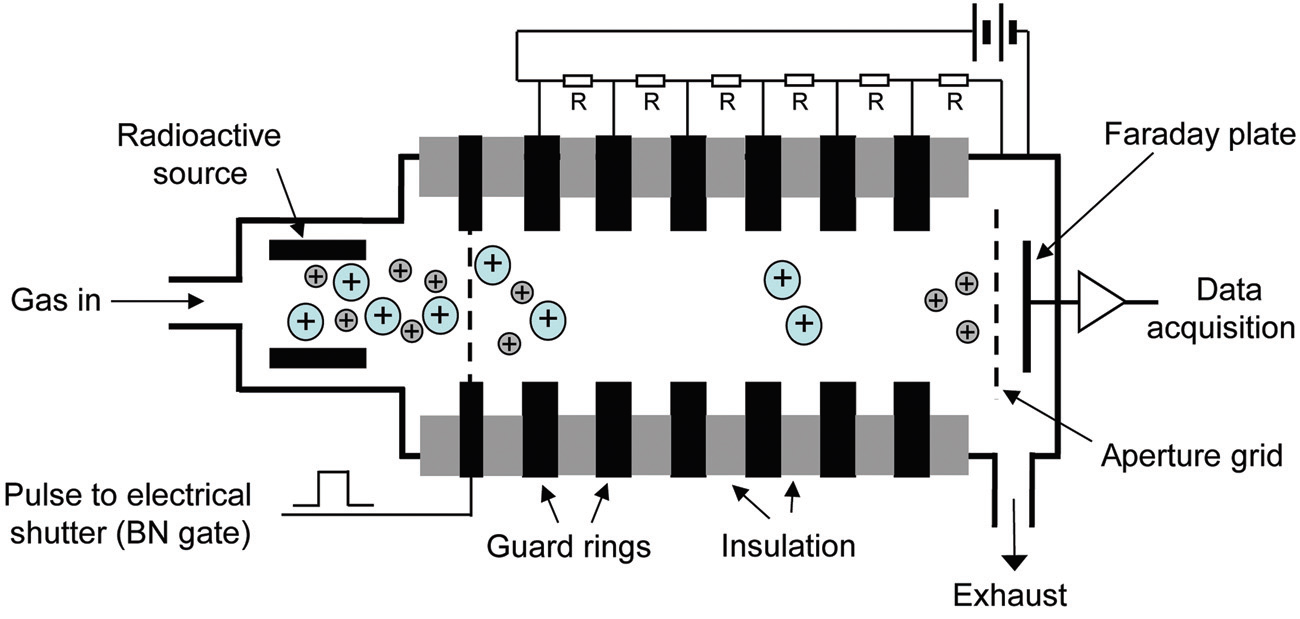
\includegraphics[width=0.65\linewidth]{pics/ims.png}
    \caption{Schematic diagram of an IMS instrument. Copyright \textcopyright  \citeauthor{ellis2013proton},  \citeyear{ellis2013proton}.}
    \label{fig:ims}
\end{figure}












\subsubsection{Selected Ion Flow Tube Mass Spectrometry}
Unlike IMS, selected ion flow tube mass spectrometry (\acrshort{sift}) does not use a drift tube, but a flow tube, to drag the ions downstream. As shown in \autoref{fig:sift}, a SIFT-MS instrument consist of an ion source, a quadrupole mass filter, a flow tube and a mass analyser.

The reagent ions (e.g. H$_3$O$^+$, NO$^+$ and O$_2^+$) are created in the ion source, which is typically a microwave resonator \cite{smith2005selected}.
Then, the quadrupole mass filter  selects the reagent ion by its mass. This piece of equipment also allows fast switching (tens of milliseconds) between the reagent ions, which can be used to extract more information of the analyte during transient experiments. From the quadrupole mass filter, the ions enter the flow tube. Here helium is used as a carrier gas and it is also in the flow tube where the analyte gas is injected. Finally, the ions are detected in a mass analyser, typically a quadrupole mass spectrometer, and the detection system builds the mass spectra obtained from the reaction of the reagent ions with the analyte.



The presence of helium in the flow tube makes it possible to explore ion-molecule reactions at thermal energies. One of the main applications of SIFT-MS is the ability to measure reaction coefficients. This has allowed SIFT-MS to become a valuable tool in areas like atmospheric and interstellar chemistry, and it has also been used as an analytical tool in other fields, being breath analysis the most remarkable one \cite{turner2006longitudinal}.

\begin{figure}%[h]
\centering
    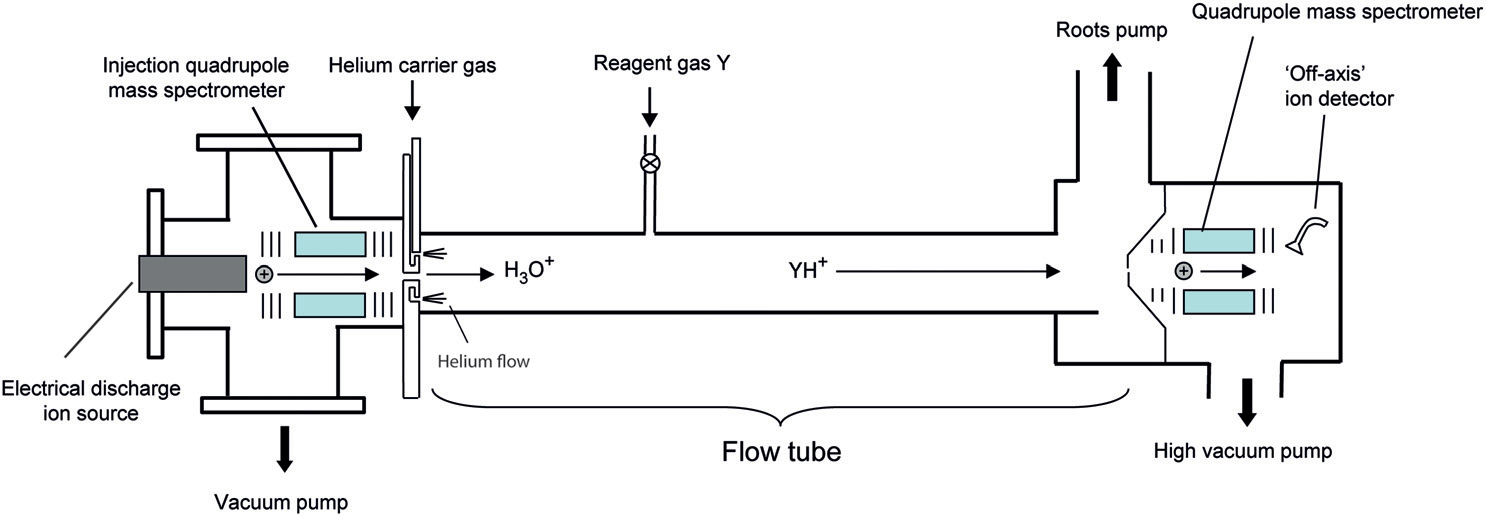
\includegraphics[width=0.95\linewidth]{pics/sift.png}
    \caption{Schematic diagram of a SIFT-MS instrument. Copyright \textcopyright  \citeauthor{ellis2013proton},  \citeyear{ellis2013proton}.}
    \label{fig:sift}
\end{figure}




\subsubsection{Proton Transfer Reaction Mass Spectrometry}
%\subsubsection{PTR-MS}
Proton transfer reaction mass spectrometry (\acrshort{ptrms}) is the main instrument used in the experimental work presented in this thesis.
It has both similarities and differences with both IMS and SIFT-MS techniques. This method was developed by Werner Lindinger at the University of Innsbruck (Austria) in the 1990 as the successor of the flowing afterglow  and the selected ion flow drift tube techniques \cite{RN601}.
The main components of a PTR-MS instrument are the ion source, the drift tube and the mass spectrometer.
Hydronium (and its water clusters) is generated in the ion source, typically a hollow cathode, from the water injected from the water reservoir. The reagent ions are then introduced into the drift tube (\acrshort{dt}). It is at this stage where they meet the analyte and proton transfer (and possible fragmentation) takes place, before the ions  are transferred then into the mass analyser, typically a time-of-flight or quadrupole mass spectrometer, for their detection. Further details of the working procedure of a PTR-MS instrument are given in the following chapter.

PTR-MS has many advantages, most of them also shared with other SCI-MS techniques. To begin with, it can detect a significant number of  VOCs such as aldehydes, ketones, aromatic compounds, alcohols,  nitriles and esters.
Because of its high sensitivity, PTR-MS can reach limits of detection of parts per quadrillion by volume (\acrshort{ppqv}) \cite{ioniconlod}.
Furthermore, reactions occurring close to the collisional rate and the possibility of directly sampling air allows for online, real-time operating conditions. Besides this, the only resources needed to run a PTR-MS instrument are distilled water and electric power.
Additionally, little or no fragmentation of the parent ions is observed, as compared to other ionisation mechanisms like EI. This  can however be manipulated to some extent by changing the conditions in the reactor. Also, selectivity can be enhanced by applying the recent instrumental developments which include, for instance, the development and implementation of an RF ion funnel \cite{barber2012increased,RF_TNT} and the use of a fast switching reduced electric field \cite{doi:10.1021/acs.analchem.7b05211}.

On the other hand, PTR-MS also has some disadvantages, being one of the most important ones the inability to directly distinguish between isomeric compounds, although this can be mitigated by using tandem MS$^n$ or fastGC techniques. % to enhance the selectivity.
Also, water cluster formation and detection can interfere with the detection of other molecules. For example, the $^{18}$O isotope of the first water cluster, (H$_2$O)H$_3$O$^+$, and the ion (C$_3$H$_3$)H$^+$ will  be both found at m/z 39. However, this issue can be solved with a high-resolution mass spectrometer and proper data analysis (e.g. using multi-peak fitting techniques or taking into account the isotopic distribution of the ions). Likewise, for compounds like benzene and toluene, which reach with H$_3$O$^+$ but not with (H$_2$O)H$_3$O$^+$, the sensitivity depends on the humidity of the air, because higher humidity means higher concentration of (H$_2$O)H$_3$O$^+$ and lower of H$_3$O$^+$. Finally, not all VOCs can be detected in PTR-MS. There exist some VOCs that don’t react with H$_3$O$^+$, like some alkanes, which have proton affinities below that of H$_2$O.












%\subsubsection{Applications of PTR-MS}
The ability of PTR-MS to detect and monitor trace concentrations of VOCs is advantageous in many fields. The main areas of application and some examples to illustrate them are:
atmospheric chemistry, where it has been used to study the emission of biogenic VOCs and their effect in the environment \cite{doi:10.1029/2003JD003863}, and to  monitor pollution and urban plumes \cite{ROGERS200626};
homeland security, where it has been  applied to  the detection of explosives \cite{RN445,RN1254,doi:10.1021/acs.analchem.7b05211}, rape drugs \cite{doi:10.1002/jms.2993}, and narcotics \cite{Agarwal2011};
in medical sciences, for the detection and monitoring of diseases through breath analysis \cite{FERNANDEZDELRIO20151243,doi:10.1152/jappl.2001.91.2.762,amann2014};
and in food sciences, to study  food aroma, flavour and quality control \cite{doi:10.1021/jf020922g,doi:10.1021/jf803998c,doi:10.1002/jms.1797}.















%\subsubsection{Advantages and disadvantages}
%Some of the advantages of most SCI-MS techniques, but in particular of PTR-MS, are:
%\begin{itemize}
%\item PTR-MS can detect a significant number of  VOCs such as aldehydes, ketones, aromatic compounds, alcohols,  nitriles and esters.
%\item Because of its high sensitivity, PTR-MS can reach limits of detection of parts per quadrillion by volume (\acrshort{ppqv}) can be achieved \cite{ioniconlod}.
%\item Little or no fragmentation of the ions, as compared to other ionisation mechanisms like electron impact.
%\item Real time measurement:
%\begin{itemize}
%\item Fast reactions, with a rate coefficient close to the collision rate, in the order of magnitude of 10$^{-9}$ cm$^{3}$/s.
%\item Direct sampling of atmospheric gases, which means that no sample preparation or pre-concentration is required.
%\end{itemize}
%\item Ease of operation, only requiring electrical power and distilled water.
%\item Sensitivity: latest instrumental developments allowed increase in sensitivity. For instance, the development and implementation of an RF ion funnel \cite{barber2012increased,RF_TNT} and the use of a fast switching reduced electric field \cite{doi:10.1021/acs.analchem.7b05211}.
%\end{itemize}

%On the other hand, PTR-MS also shows the following disadvantages:
%\begin{itemize}
%\item Inability to directly distinguish isomeric compounds. This can be mitigated by using tandem MS$^n$ or fastGC techniques to enhance the selectivity.

%\item Water cluster formation and detection can interfere with the detection of other molecules. For instance, the $^{18}$O isotope of the first water cluster, (H$_2$O)H$_3$O$^+$, and the ion (C$_3$H$_3$)H$^+$ will  be both found at m/z 39. However, this issue can be solved with a high-resolution mass spectrometer and proper data analysis, i.e. using multi-peak fitting techniques or taking into account the isotopic distribution of the ions.

%\item For compounds like benzene and toluene, which do not react with (H$_2$O)H$_3$O$^+$, the sensitivity depends on the humidity of the air, because higher humidity means higher concentration of (H$_2$O)H$_3$O$^+$ and lower of H$_3$O$^+$.

%\item There exist some VOCs that don’t react with H$_3$O$^+$, like some alkanes, which have proton affinities below that of H$_2$O, so the back reaction (equation \ref{eq:ptb}) is not negligible. %Isoflurane also has a lower proton affinity lower than that of water, but product ions are observed.
%\end{itemize}





%\begin{itemize}
%\item Atmospheric chemistry:
%\begin{itemize}
%\item Determination of the emission of biogenic VOCs and their effect in the environment \cite{doi:10.1029/2003JD003863}.
%\item Monitoring of pollution and urban plumes \cite{ROGERS200626}.
%\end{itemize}
%\item Homeland security:
%\begin{itemize}
%\item Detection of explosives \cite{RN445,RN1254,doi:10.1021/acs.analchem.7b05211}, rape drugs \cite{doi:10.1002/jms.2993} and narcotics \cite{Agarwal2011}.
%\end{itemize}
%\item Medical sciences:
%\begin{itemize}
%\item Detection and monitoring of diseases through breath analysis \cite{FERNANDEZDELRIO20151243,doi:10.1152/jappl.2001.91.2.762,amann2014}.
%\end{itemize}
%\item Food sciences:
%\begin{itemize}
%\item Study of food aroma and flavour and quality control cite{doi:10.1021/jf020922g,doi:10.1021/jf803998c,doi:10.1002/jms.1797}.
%\end{itemize}
%\end{itemize}





























\section{Thesis outline}
In the first chapter I present an introduction to soft chemical ionisation mass spectrometry together the outline  and the aim of the present thesis.

% 2 PTRMS

In the second chapter, the PTR-MS technique %, its underlying chemistry
and relevant experimental aspects are explained in detail.

% 3 cocaine
% 4 other drugs
The first chapter including experimental work is the third one, where cocaine and related compounds of interest are investigated, including results from both PTR-MS and density functional theory calculations.

The fourth chapter  carries on with the same topic, with PTR-MS results from the measurements of other illicit drugs of common societal abuse.

% 5 RF nitros
The fifth chapter is an adapted version of my  paper regarding the enhancement of selectivity in the detection of %nitro-, dinitro- and trinitrotoluenes
explosives
through the implementation of an RF ion funnel in the reactor of a PTR-ToF-MS.

% 6 nitroanilines
The sixth chapter is a reformatted version of my  paper about the use selective reagent ion mass spectrometry for the study of nitroanilines isomers.

% 7 phthalates
The seventh chapter is an adapted version of my  paper regarding the investigations of phthalates in PTR-MS using direct headspace sampling.

% 8 ketones
The eighth chapter is a rewritten version of my  paper of relevance to breath analysis about the study of ketones using a fastGC-PTR-ToF-MS instrument %at  different humidities.
in dry and humid conditions.

% 9 conclusions
In the ninth chapter the final conclusions and closing remarks are stated.

%In the appendices I include papers, other data that didn't fit in the thesis, etc



\section{Aim of the thesis}
My research project was focused on the study of ion-molecule interactions in the reaction region of proton transfer reaction mass spectrometry,  mainly in the area of homeland security, but other applications have also been investigated, including a study of ketones of relevance to breath analysis.

Compounds of specific interest for my research are  illicit drugs, explosives and phthalates. The available studies, if any, had been done at only one reduced electric field (typically between 120 – 140 Td). The experimental work in this thesis  is supplemented by quantum chemical calculations, which are used to help interpret the results. These were conducted using Gaussian09W and GaussView05 for Windows by Dr Peter Watts. All calculations used the B3LYP hybrid functional and the 6-31+G(d,p) basis set.

The main outcome of this thesis has strengthened knowledge of ion-molecule interactions in \acrshort{scims} techniques, in collaboration with other research groups and institutions within the Marie Sk\l{}odowska-Curie Actions Innovative Training Network IMPACT: Ion-Molecule Processes for Analytical Chemistry Technologies (\href{www.impact-h2020itn.com}{www.impact-h2020itn.com}) funded by the European Commission’s HORIZON 2020 Programme under Grant Agreement Number 674911.


%At least three publications are expected as first author as well as other publications from collaborations as second or third author.
%The planned secondments and trainings in other institutions have taken place.


% OLD

%\texttt{The topic of my thesis is the underpinning of ion-molecule processes and their use as analytical probes in soft chemical ionisation mass spectrometry (SCIMS). This includes studying specific ion-molecule reaction processes and their dependence on temperature, reduced electric field, pressure, etc. This is being done in the field of homeland security, in particular to illicit drugs. I am also interested in studying the implementation of a radio frequency ion funnel in PTR-MS to enhance selectivity and sensitivity, and the use of a thermal desorption unit as method to detect semi volatile organic compounds. Moreover, I want to use computational methods to study the trajectories of ions inside the reactor of a PTR-MS instrument at different experimental conditions to gain knowledge about the transmission of ions to the subsequent stages of a PTR-MS instrument. Furthermore, I am one of the ten early stage researchers (ESRs) of the IMPACT network (see appendix).}








